\chapter{\kadaid}
\section{\purpose}
我々は,ポスターなどの写真を注視するとき,どこをよく見るだろうか.どこを注視しているか追跡する技術を「アイトラッキング技術」と呼ぶが,この技術はマーケティングの分野にも応用されている.
金融機関店舗における利用者の注視行動の調査\cite{アイトラッキング技術を用いた地域実践的研究の報告}では,注視したとされるものは印象に残ることが分かっている.
この実験では,人の顔,指差し,文字が含まれたポスターに対して眼球運動を計測する.ポスター中のどこを注視しているかを定量化し,注意の向け方について考察する.

\begin{wrapfigure}{r}[0mm]{.15\textwidth}
    \centering
    \includegraphics[keepaspectratio,width=.15\textwidth]{../../12_DataAnalysis/snapshot.jpg}
    \caption{注視画像}
    \label{fig:注視画像}
    \vspace{-1.5cm}
\end{wrapfigure}
\section{\method}
今回は,アイトラッキングするための装置としてTobii社の\tobi を用いる.注視する対象として\figref{fig:注視画像}を用いる.
この実験の参加者は,学生の20代男性1名である.実験手続を以下に示す.
\begin{enumerate}
    \renewcommand{\labelenumi}{\fbox{\theenumi}}
    \item \tobi のメガネを装着する.
    \item 呈示されるマーカを追視し,視線方向のキャリブレーションを行う.
    \item 刺激(\figref{fig:注視画像})を自由に観察したときのGaze Plot,Heat Mapを作成する.
\end{enumerate}
\paragraph{Gaze Plot}
数値と円の大きさで,注視た順番と注視た時間を表現するグラフである.
数値は,注視した順番を表す.円の大きさは注視した時間を表す.円の大小と,注視時間は比例関係にある.
また,注視した順番が表示されるので,目線の軌跡も分かる.

\begin{wrapfigure}{o}[0mm]{.42\textwidth}
    \centering
    \begin{minipage}[b]{.2\textwidth}
        \centering
        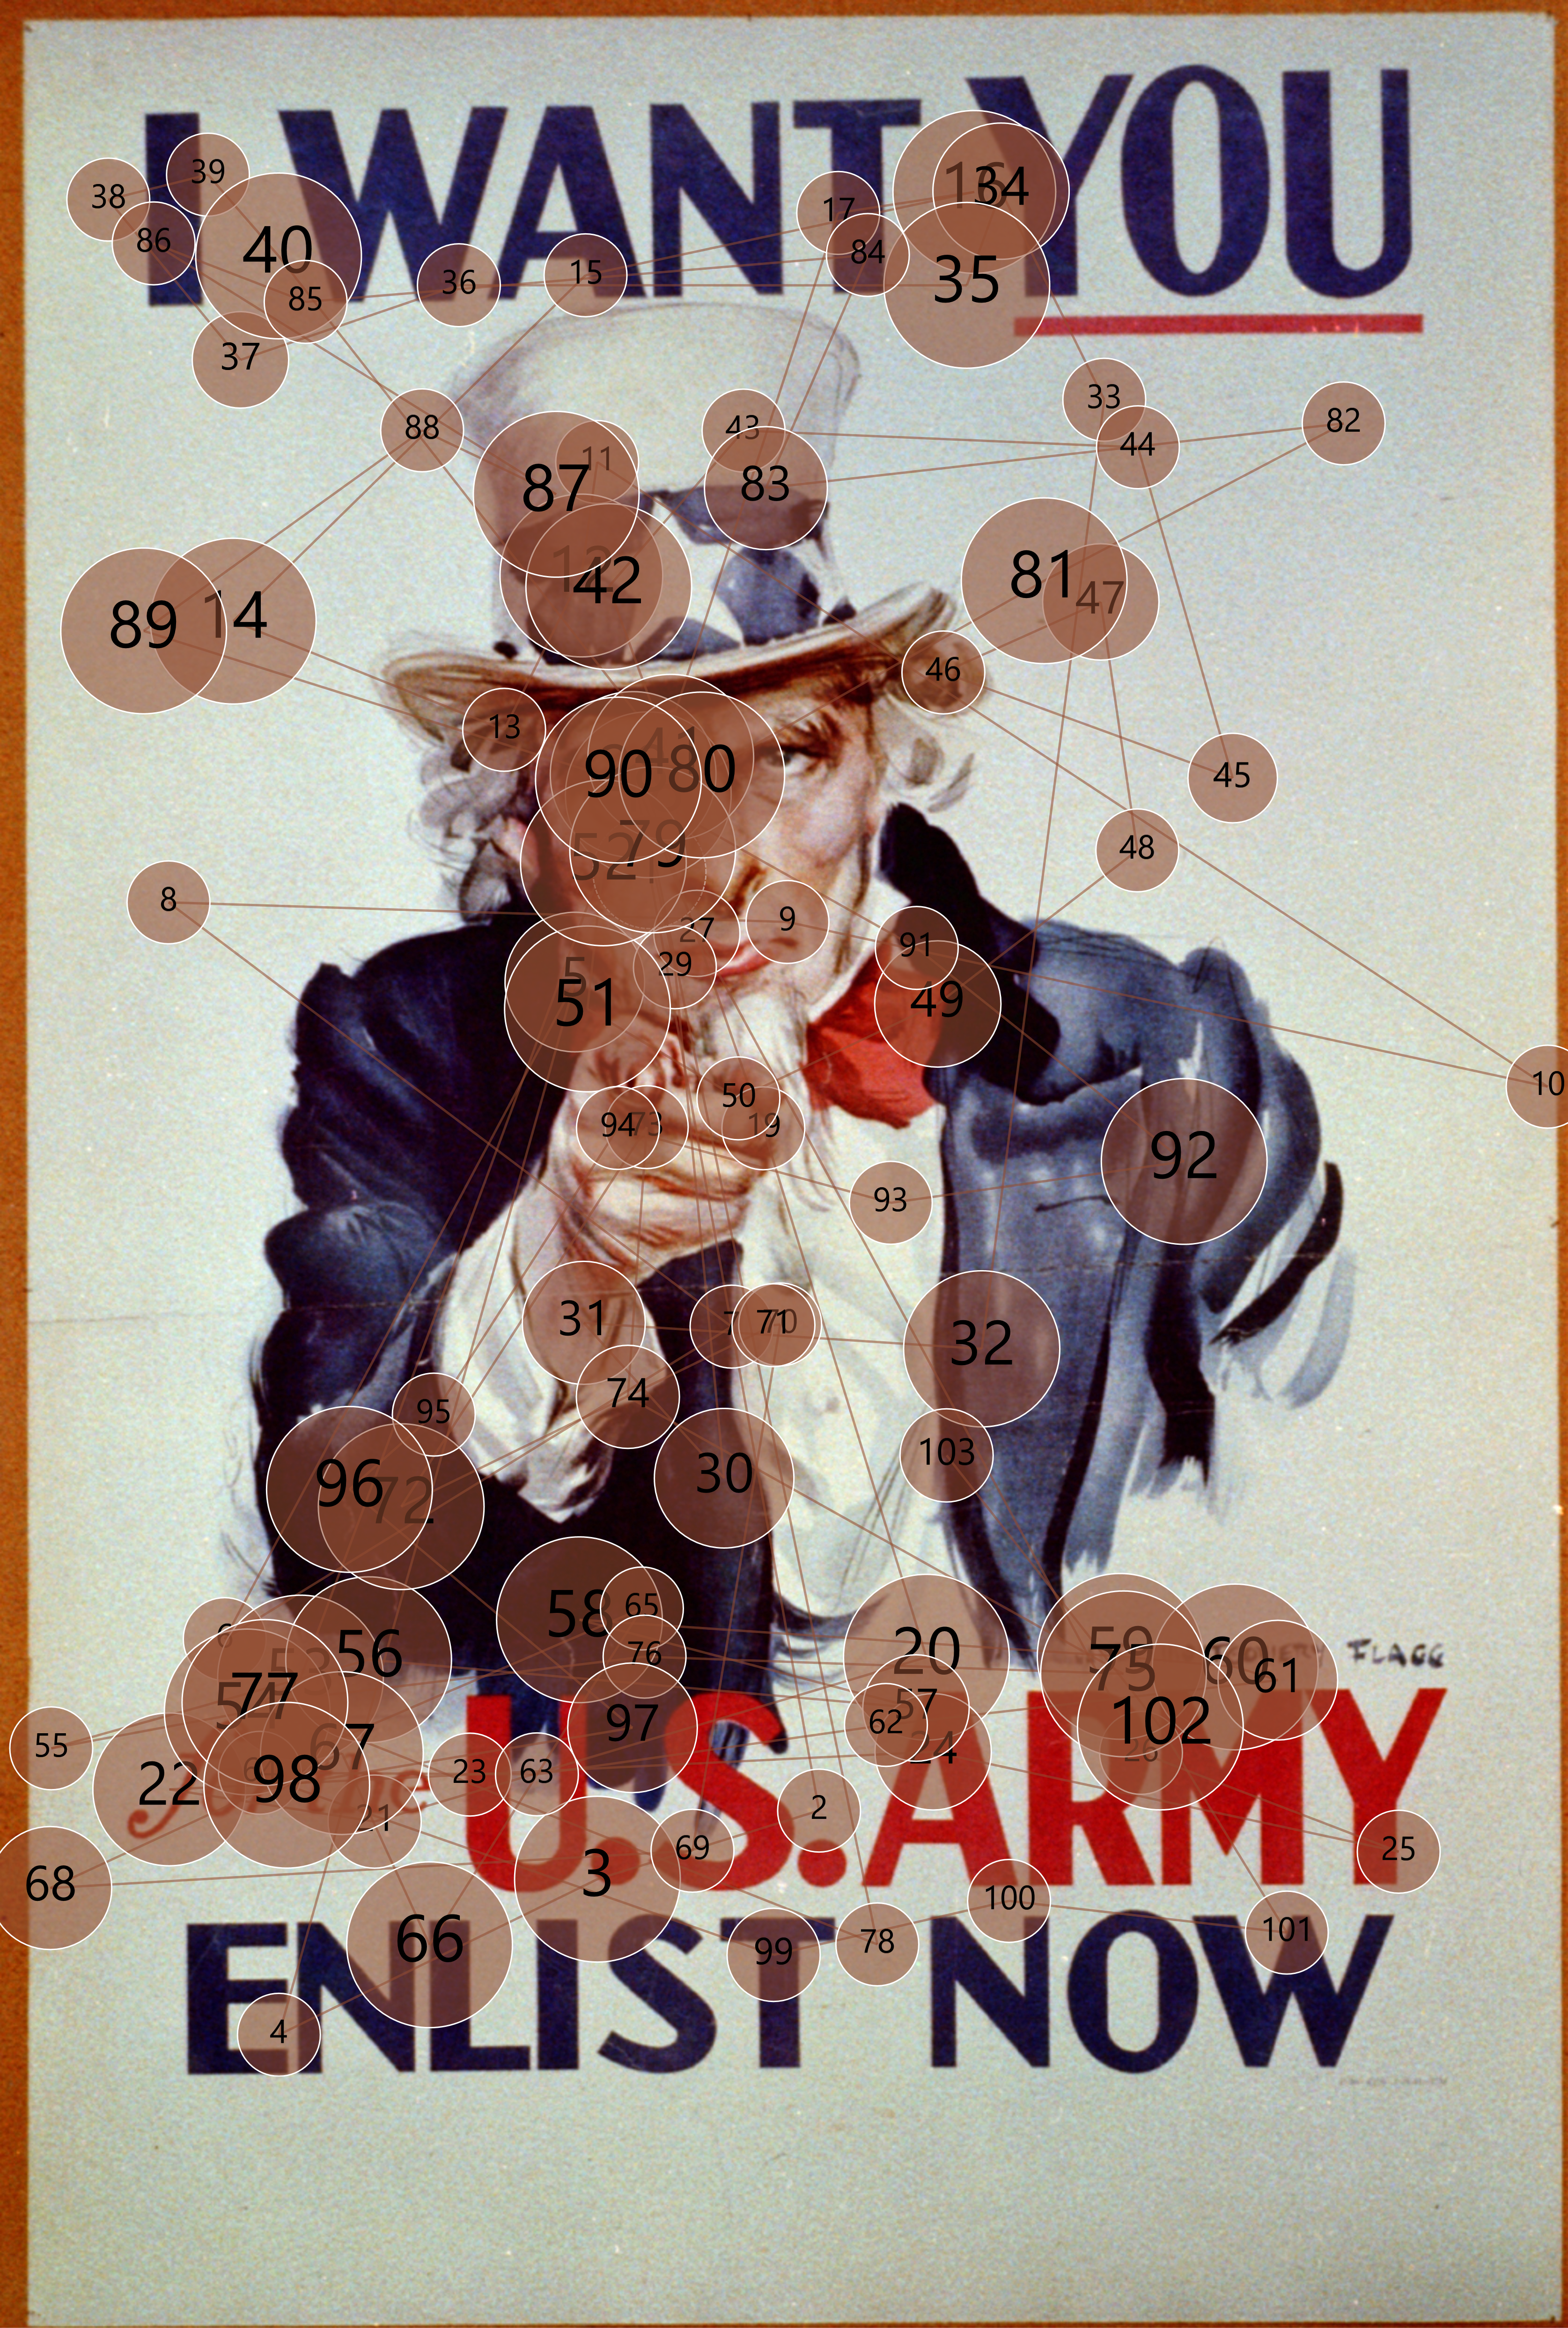
\includegraphics[keepaspectratio,width=\textwidth]{../../12_DataAnalysis/GazePlot.png}
        \subcaption{Gaze Plot}
    \end{minipage}
    \begin{minipage}[b]{.2\textwidth}
        \centering
        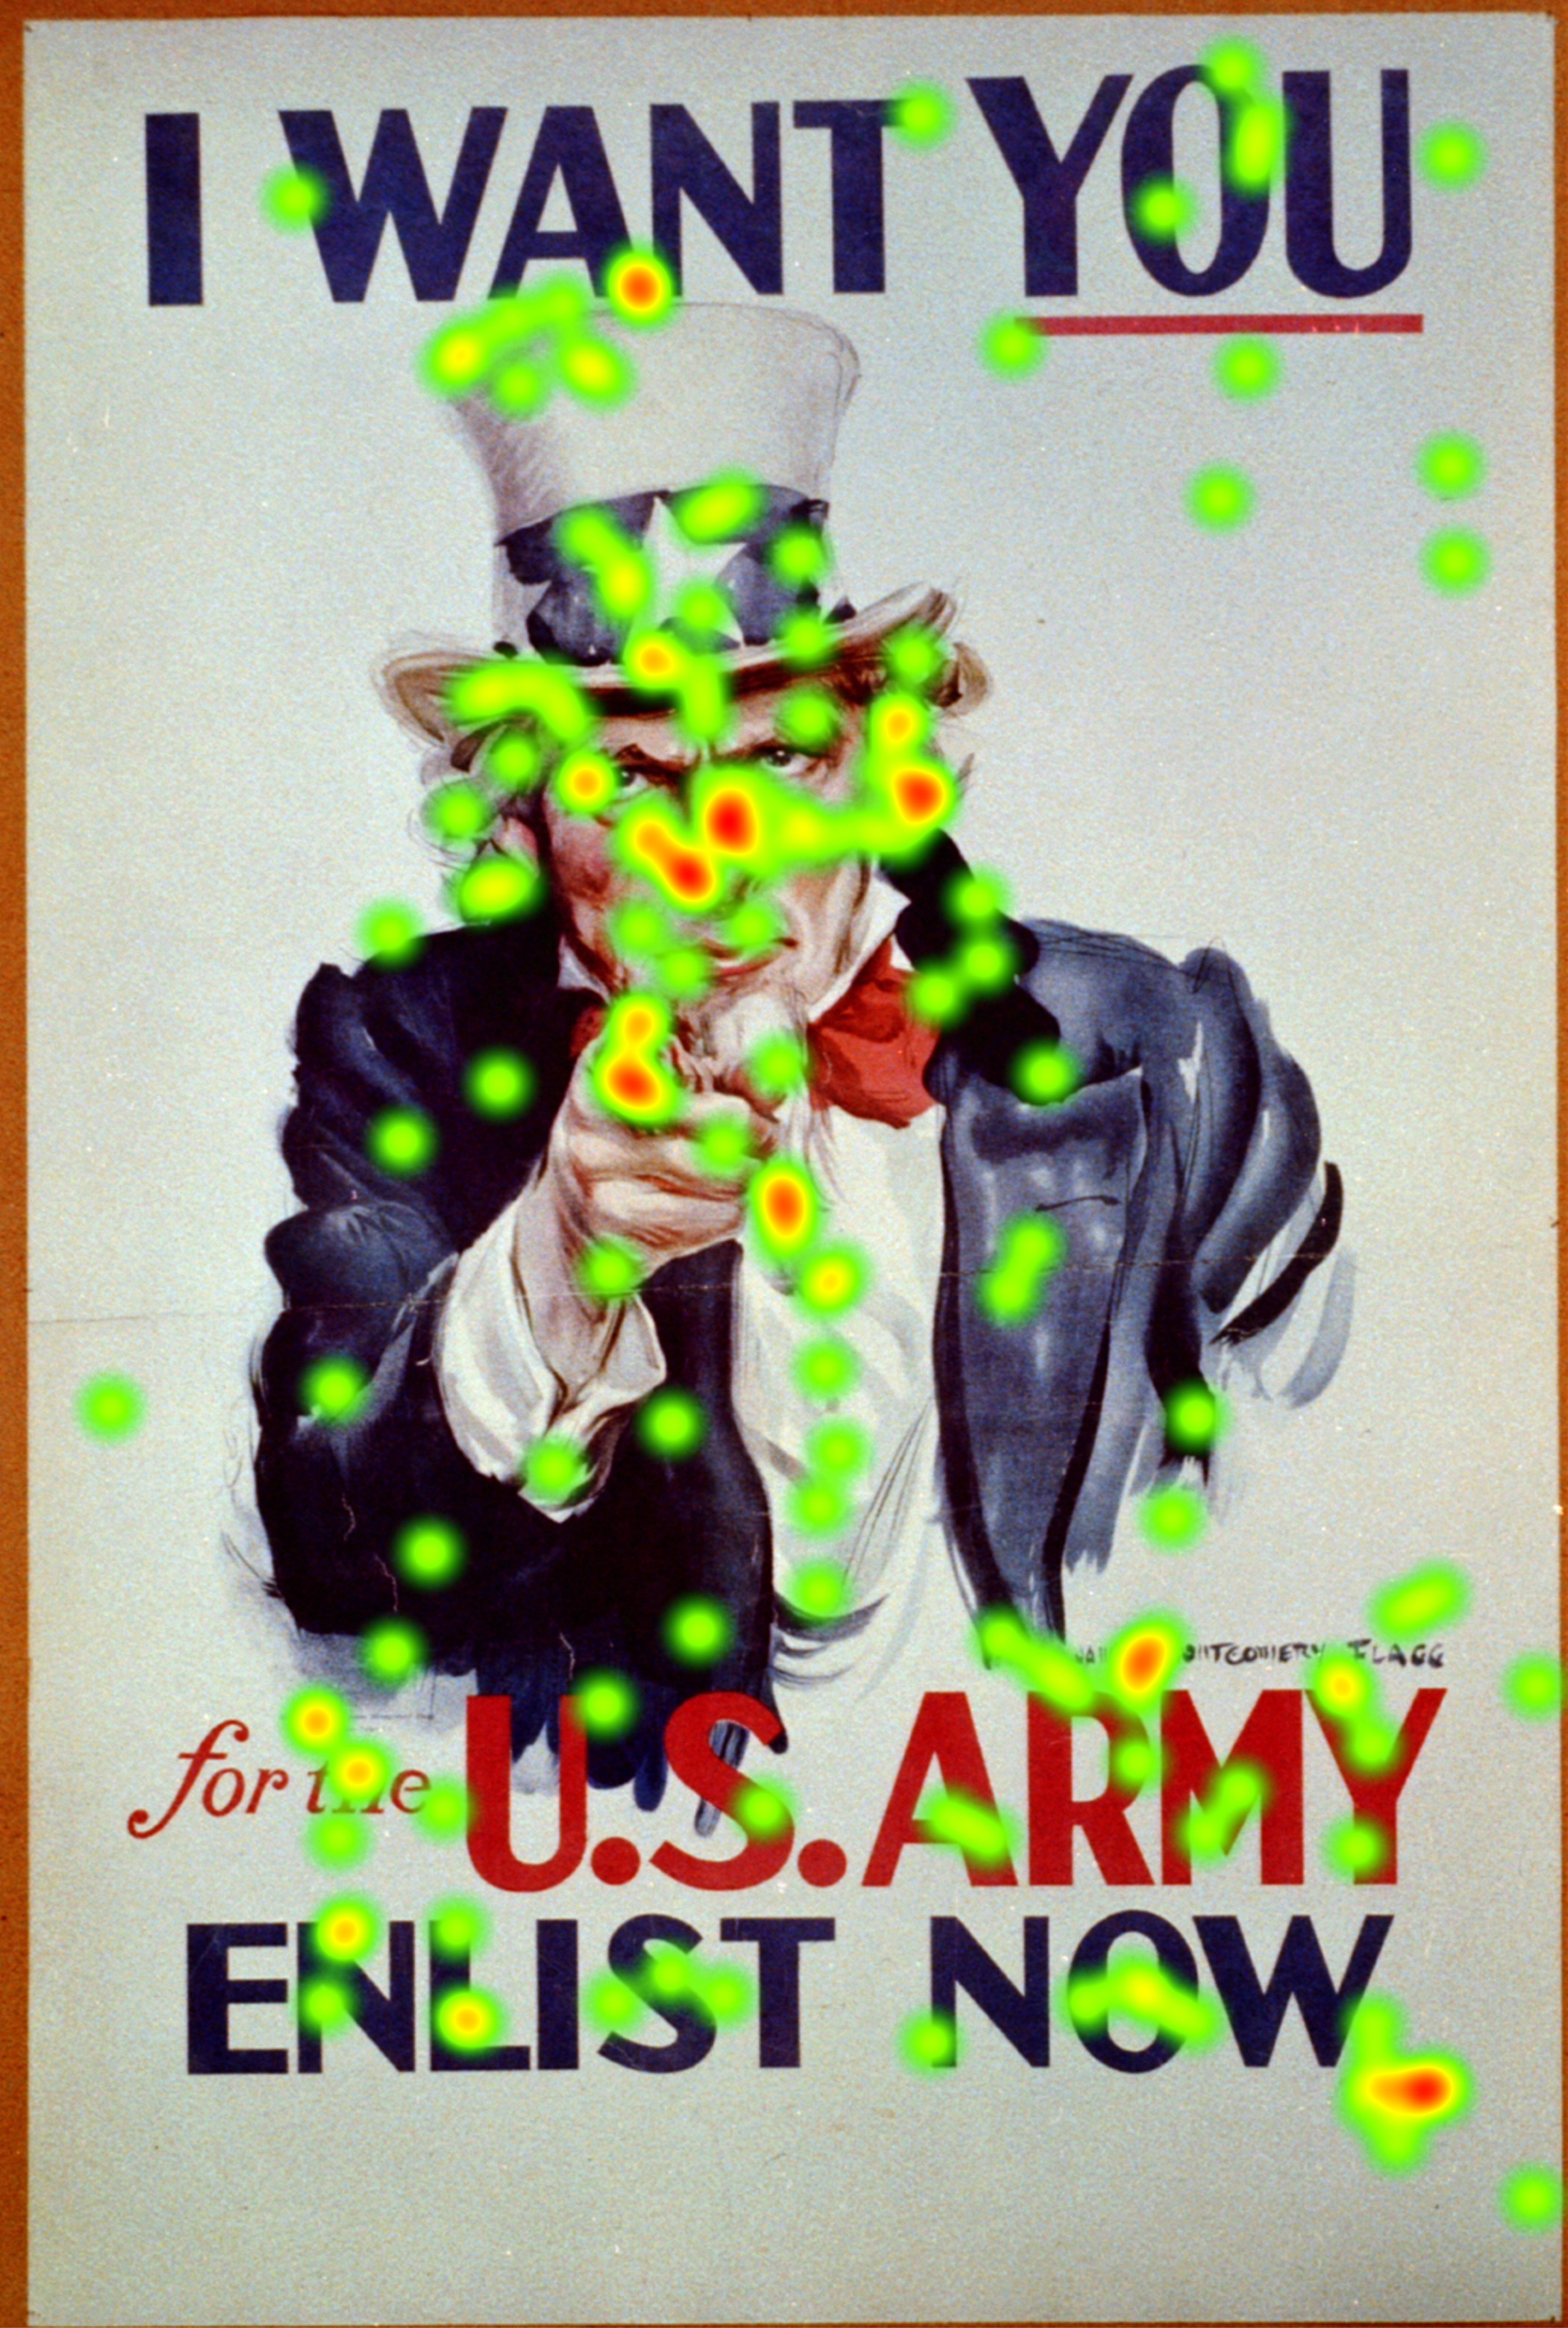
\includegraphics[keepaspectratio,width=\textwidth]{../../12_DataAnalysis/HeatMap.png}
        \subcaption{Heat Map}
    \end{minipage}
    \caption{\kadaid 実験結果}
    \label{fig:実験結果\kadaid}
\end{wrapfigure}
\paragraph{Heat Map}
注視時間が長い箇所を赤く表示する図である.
\section{\result}
作成したGaze PlotおよびHeat Mapを\figref{fig:実験結果\kadaid}に示す.
\section{\consideration}
